\documentclass[prl,twocolumn,superscriptaddress,float,aps]{revtex4-2}
\usepackage{bm,color,amsmath,amssymb,mathrsfs,latexsym,graphicx,psfrag,tabularx}
\usepackage[hidelinks,colorlinks,linkcolor=blue,citecolor=blue,urlcolor=blue]{hyperref}
\usepackage{etoolbox}
\makeatletter
\patchcmd{\@maketitle}{\@author}{\@author\show\@thanks}{}{}
\makeatother
\usepackage{dsfont}
\usepackage{xcolor}
\usepackage{enumitem}

% ── Custom Commands (merged) ──────────────────────────────────
\newcommand{\ii}{\mathrm{i}}
\newcommand{\dd}{\mathrm{d}}
\newcommand{\kk}{\mathbf{k}}
\newcommand{\rr}{\mathbf{r}}
\newcommand{\tr}{\operatorname{tr}}
\newcommand{\Lmax}{N_{\max}}

\newcommand{\bra}[1]{\langle #1|}
\newcommand{\ket}[1]{|#1\rangle}
\newcommand{\braket}[2]{\langle #1|#2\rangle}

\newcommand{\ELLminus}{E^{\uparrow}_{-}}
\newcommand{\ELLplus}{E^{\uparrow}_{+}}
\newcommand{\ELLTRminus}{E^{\downarrow}_{-}}
\newcommand{\ELLTRplus}{E^{\downarrow}_{+}}
\newcommand{\ELLzero}{E^{\uparrow}_{0}}
\newcommand{\ELLTRzero}{E^{\downarrow}_{0}}
\newcommand{\ELLpm}{E^{\uparrow}_{\pm}}
\newcommand{\ELLTRpm}{E^{\downarrow}_{\pm}}

\newcommand{\hOmega}{\widetilde{\Omega}}
\newcommand{\homega}{\widetilde{\omega}}
\newcommand{\hM}{\widetilde{M}}
\newcommand{\meff}{m^{*}_{\mathrm{eff}}}
\newcommand{\Bstar}{B^{*}}
\newcommand{\dmu}{\delta\mu}

\newcommand{\Berry}{\Omega}
\newcommand{\metric}{g}

\newcommand{\Eflat}{E_{\mathrm{flat}}}
\newcommand{\Etop}{E_{\mathrm{top}}}
\newcommand{\kB}{k_{\!B}}

\newcommand{\cref}[1]{ref.~\ref{#1}}
\newcommand{\Cref}[1]{Ref.~\ref{#1}}

\newcommand{\bs}[1]{\boldsymbol{#1}}
\newcommand{\abs}[1]{\left|#1\right|}
\newcommand{\re}{\mathrm{Re}}
\newcommand{\im}{\mathrm{Im}}
\newcommand{\expect}[1]{\left\langle#1\right\rangle}

\newcommand{\commentCXL}[1]{{\color{red} \footnotesize (\textsf{Chaoxing}) \textsf{\textsl{[#1]}}}}

\begin{document}

\title{Lifshitz--Kosevich Theory of Anomalous Landau Levels in Topological Flat Bands}
\author{Chao-Xing Liu}
\affiliation{%
	Department of Physics, The Pennsylvania State University, University Park, Pennsylvania 16802, USA
}
\affiliation{Center for Theory of Emergent Quantum Matter, The Pennsylvania State University, University Park, Pennsylvania 16802, USA}
\date{\today}

\begin{abstract}
	In conventional metals, quantum oscillations arise from Landau quantization of Fermi-surface cyclotron orbits, whose dynamics are governed by the Fermi velocity and cyclotron effective mass within Lifshitz--Kosevich (LK) theory. A perfectly flat band, by contrast, has vanishing group velocity, which would na\"ively imply an infinite cyclotron mass and complete thermal suppression of quantum oscillations. Yet topological flat bands can support anomalous Landau levels (LLs) whose finite-field spacing is generated by quantum geometry rather than band curvature, allowing quantum oscillations to persist. This work addresses how such anomalous flat-band LLs behave within the LK framework and whether their thermal damping can reveal quantum-geometric information. Using a minimal model with exactly flat topological bands, we derive an LK theory for these anomalous LLs and analyze fixed-density magnetization oscillations. The resulting oscillations exhibit a finite LK effective mass that is substantially larger than the normal-band value and possesses a strong magnetic-field dependence. In the weak-field limit, this anomalous mass reflects the quantum-geometric origin of the LL spacing and scales inversely with both the magnetic field and the trace of the quantum metric. Thus, thermal damping of flat-band quantum oscillations directly measures the quantum metric, establishing quantum oscillations as a probe to flat-band quantum geometry.
	%Yet topological flat bands support anomalous Landau levels (LLs) whose spacing is generated at finite magnetic field by quantum geometry rather than band curvature, so finite oscillations persist.
	%	This paper addresses two concrete questions: \emph{(i) how do quantum oscillations of anomalous flat-band LLs behave within the LK framework, and (ii) can quantum geometric information be extracted from their thermal damping?}
	%	Working with the topological heavy-fermion (THF) model, a minimal two-band system that hosts an exactly flat, topological lower band, we derive an LK theory in which the thermal damping scale is set by the \emph{local} LL spacing $v_\mu = |\partial E/\partial n|$ at the Fermi level, not by a band-averaged cyclotron energy.
	%	A fixed-density magnetization analysis of normal and anomalous regimes, with effective masses extracted from harmonic LK fits, gives two clean answers.
	%	\emph{(i)} Anomalous LLs produce finite oscillations whose thermal damping is governed by $v_\mu$; in the conventional effective-mass language this yields an anomalous mass an order of magnitude larger than the normal-band value and strongly field-dependent.
	%	\emph{(ii)} In the weak-field limit the local spacing reduces to $|\partial E/\partial n| \sim a B^2 \tr g$, so that $\meff \sim 1/(a B\,\tr g)$: the LK thermal scale directly probes the integrated quantum metric of the flat band, providing an experimental route from quantum-oscillation thermal damping to quantum-geometric content.
\end{abstract}

\maketitle

%% ================================================================
% ================================================================
% \section{Introduction}
% \label{sec:intro}
% ================================================================

%Quantum oscillations of thermodynamic and transport quantities in a magnetic field are among the most direct probes of a metal's Fermi surface.
{\it Introduction - }
Quantum oscillations are conventionally understood as a Fermi-surface phenomenon~\cite{shoenberg1984magnetic}: in a magnetic field, cyclotron orbits are quantized into Landau levels, and their passage through the Fermi energy produces oscillatory thermodynamic and transport responses. 
The standard Lifshitz--Kosevich (LK) formalism~\cite{lifshitz1956theory,shoenberg1984magnetic} expresses
the oscillatory part of the grand potential $\delta \Omega$ at a finite temperature as a sum over harmonics,
\begin{equation}
	\delta \Omega \propto \sum_{p=1}^{\infty}
	\frac{R_T(p)}{p^{2}}
	\cos (2\pi p\,F/B - \phi),
	\label{eq:lk-standard}
\end{equation}
where $p$ is the harmonic index, $F$ and $\phi$ define the oscillation frequency and phase, respectively, and $B$ is external magnetic field. The thermal damping factor $R_T(p) = X_p/\sinh X_p$ depends on
$X_p = 2\pi^{2} p \kB T / \hbar\omega_{c}$, with the cyclotron energy
$\hbar\omega_{c} = e\hbar B / m^{*}$ set by the cyclotron mass $m^{*}$, which
therefore fixes the characteristic temperature scale of thermal smearing. In
systems with vanishing band dispersion, however, the band mass diverges.
Applied literally to a perfectly flat band, $m^{*}\!\to\!\infty$ gives
$X_p\!\to\!\infty$ and $R_T\!\to\!0$, so the conventional LK formula predicts
complete thermal suppression and a total absence of quantum oscillations. This conclusion, however, rests on identifying the thermal damping scale with a
cyclotron energy set by the band dispersion---an identification that need not hold
for topological flat bands, which have recently been realized in moir\'e materials~\cite{bistritzer2011moire,cao2018unconventional,serlin2020intrinsic,song2022magic,ledwith2020fractional,cai2023signatures,zeng2023thermodynamic,xu2023observation,adak2024tunable,mak2022semiconductor,balents2020superconductivity,liu2021orbital,checkelsky2024flat,torma2022superconductivity,song2019all,song2021twisted,po2019faithful,ahn2019failure}. Whether quantum oscillations persist in such a band,
and how the LK damping factor should be reformulated when the conventional dispersive cyclotron energy is absent, remain unresolved.

Recently, it was recognized that the Landau levels of a perfectly flat band under magnetic fields may not remain degenerate but instead can spread over a finite energy window. The magnitude of this anomalous Landau-level spreading is set by the quantum geometry of the Bloch states~\cite{kang2025measurements,kim2025direct,yu2025quantum,torma2023essay,liu2025quantum} ---quantified by the Hilbert--Schmidt quantum distance and the cross-gap Berry connection---rather than by any band dispersion~\cite{rhim2020quantum,hwang2021geometric,rhim2020singular,long2026interplay,jung2024quantum,kawakami2025singular,datta2025anomalous,fu2026anomalous}.
This spreading endows even a perfectly flat band with a finite, field-dependent energy scale that has no counterpart in the dispersive cyclotron picture, reopening the possibility that quantum oscillations survive in the flat-band limit---now controlled by quantum geometry rather than by band curvature.
This raises two questions for topological flat bands: what replaces the
cyclotron energy in the LK thermal damping of anomalous LL oscillations, and
can that damping be used to extract quantum-geometric information?

To address these questions, we develop an LK theory for quantum oscillations of anomalous LLs in a minimal model with perfectly flat topological bands~\cite{liu2025ideal}. Our central claim is that the LK thermal damping for anomalous LL oscillations is controlled by the \emph{local} LL spacing at the Fermi level, $v_\mu^{\alpha,\eta}=\bigl|\partial E^\alpha_\eta(n,B)/\partial n\bigr|_{n^*_{\alpha,\eta}}$, where $E^\alpha_\eta$ is the branch-resolved Landau-level energy and $n$ is the Landau-level index treated as a continuous variable. We compare fixed-density magnetization oscillations of normal LLs, associated with dispersive bands, with anomalous LLs from topological flat bands. We compute their temperature dependence, extract the thermal damping from local oscillation windows, and express the results in the conventional effective-mass framework. Although the anomalous LL oscillations exhibit much stronger thermal damping, the fitted effective masses remain finite, are approximately an order of magnitude larger than the normal-band masses in the representative comparison, and exhibit a clear monotonic field dependence, in contrast with the nearly constant normal-band masses. Expanding the exact LL spacing in the weak-field limit yields $v_\mu^{\alpha,-} \sim B^2 \tr\metric$, so that $\meff \sim 1/(B\,\tr\metric)$, where $B$ is the magnetic field and $\metric$ is the quantum metric. The LK thermal scale of anomalous oscillations is thus directly tied to the quantum metric of the topological flat band. Taken together, these results answer both questions: \emph{(i)} anomalous flat-band oscillations persist within the LK framework, with the local LL spacing $v_\mu^{\alpha,\eta}$ replacing the cyclotron energy and yielding a finite, strongly field-dependent effective mass larger than the dispersive-band value; and \emph{(ii)} their thermal damping provides a probe of flat-band quantum geometry.

% % ================================================================
% \section{Landau Levels of Ideal Topological Flat Bands}
% \label{sec:model}
% % ================================================================

{\it Ideal topological flat bands - } We start with a minimal model with perfectly flat topological bands, which can describe low-energy physics of moir\'e heterostructures with type-II band alignment in Ref.~\cite{liu2025ideal}. This model consists of heavy (flat) fermion and light (dispersive) fermion components, 
% ~\cite{song2022magic}, 
and the corresponding Hamiltonian is given by 
\begin{equation}
	H_\alpha(\kk) =
	\begin{pmatrix}
		E_0 + a k^{2} & \alpha c k_{\alpha} \\
		\alpha c k_{-\alpha}    & E_0 + \Delta_f
	\end{pmatrix},
	\label{eq:thf-hamiltonian}
\end{equation}
where $\alpha=\uparrow, \downarrow$ or $\pm$ labels two opposite spin states, $k_{\pm} = k_x \pm \ii k_y$, $a$ defines the band-curvature coefficient of the dispersive bands, $c$ is the coupling between the flat and dispersive bands, and $E_{0}$ is the energy reference and $\Delta_f$ is the energy separation between the flat and dispersive bands at $\kk=0$. The above Hamiltonian is valid within the momentum cutoff $\Lambda$, e.g. $|\kk| \le \Lambda$, which is set by the moir\'e Brillouin zone size in moir\'e heterostructures. In our numerical results, energies and the thermal scale $k_B T$ are measured in $\mathrm{eV}$ and lengths in $\mathrm{nm}$. 
% Thus, $k$ and $\Lambda$ are measured in $\mathrm{nm}^{-1}$, $B$ and $\rho$ in $\mathrm{nm}^{-2}$, $a$ in $\mathrm{eV\cdot nm}^{2}$, and $c$ in $\mathrm{eV\cdot nm}$. 
Two spin Hamiltonians $H_\uparrow$ and $H_\downarrow$ are related by time-reversal (TR) symmetry, e.g. $H_\downarrow(\kk) = H_\uparrow^*(-\kk)$, so the full system satisfies TR. When the condition $\Delta_f = \frac{c^{2}}{a}$ is satisfied, the lower band is perfectly flat with $E^{\uparrow (\downarrow)}_{-}(\kk) = E_0$ and the upper band is dispersive with a finite gap, given by $E^{\uparrow (\downarrow)}_{+}(\kk) = E_0 + \frac{c^{2}}{a} + a k^{2}$, as shown in Fig.~\ref{fig:main1}a. The full effective Hamiltonian possesses both TR and inversion symmetries, so the eigen-states for spin up and down Hamiltonian are degenerate at each momentum. For the perfectly flat lower band $E^{\uparrow (\downarrow)}_-$, its wavefunction carries nontrivial quantum geometry, as demonstrated by the Berry-curvature distribution in Fig.~\ref{fig:main1}b. In particular, the lower band satisfies the ideal quantum geometry condition
\begin{align}
	\tr\metric_{\alpha}(\kk) = |\Berry_{\alpha}(\kk)|
	= \frac{2c^{2}}{(a k^{2} + c^{2}/a)^{2}}.
	\label{eq:geometry-results}
\end{align}
Thus, the two TR-related sectors have the same quantum metric and opposite Berry curvature; the spin-up (spin-down) flat band has Chern number $+1$ ($-1$).
More discussion on the quantum geometry of ideal topological flat bands can be found in Sec.A of Supplementary Materials (SM). 

% The quantum geometric tensor for an isolated band is $Q_{ij}=\langle \partial_i u_{-}|u_{+}\rangle\langle u_{+}|\partial_j u_{-}\rangle$.
% Using the Hellmann--Feynman relation and the explicit states, one finds (see the Supplementary Material for the full calculation)
% \begin{align}
% 	\metric_{xx} = \metric_{yy} & = \frac{c^{2}}{(a k^{2} + c^{2}/a)^{2}},\qquad
% 	\metric_{xy}=0,                                                              \\
% 	\Berry                      & = \frac{2c^{2}}{(a k^{2} + c^{2}/a)^{2}},
% 	\label{eq:geometry-results}
% \end{align}
% satisfying the ideal-geometry condition $\tr\metric(\kk)=\Berry(\kk)$.
% This condition means that at every momentum the band saturates a topological bound and has minimal quantum-metric spread; the sharp Berry-curvature peak at $\kk=0$ in Fig.~\ref{fig:main1} is its direct manifestation.

% The integrated metric $T\equiv\int_{|\kk|\le\Lambda}\tr\metric(\kk) \frac{d^{2}k}{(2\pi)^{2}}$ evaluates to $T = a\Lambda^{2}/[2\pi(a\Lambda^{2}+c^{2}/a)]$, approaching $1/(2\pi)$ as $\Lambda\to\infty$, consistent with Chern number $C=+1$.

% \subsection{Landau-level spectrum}
% \label{sec:model-LL}

We next consider this minimal model under a perpendicular magnetic field $\mathcal{B}$, which enters through minimal coupling $\kk\to\boldsymbol{\Pi} = \kk + e\mathbf{A}/\hbar$, where $\mathbf{A} = \frac{\mathcal{B}}{2}(-y,x,0)$ is the vector potential for the symmetric gauge.
The canonical momentum operators satisfy $[\Pi_x,\Pi_y]=-\ii B$ with $B = e\mathcal{B}/\hbar$, so the ladder operators can be defined as $b = \Pi_-/\sqrt{2B}$, $b^{\dagger} = \Pi_+/\sqrt{2B}$ with $[b,b^{\dagger}]=1$. Here, \(B\) is measured in \(\mathrm{nm}^{-2}\). Using these operators, we solve the Hamiltonian in Eq.~\eqref{eq:thf-hamiltonian} (see SM Sec.~B). The spectrum in Fig.~\ref{fig:main1}(c) comprises two zeroth LLs,
\begin{equation}
	\ELLzero(B) = E_0 + aB,\qquad
	\ELLTRzero(B) = E_0 + \frac{c^{2}}{a} = E_0 + \Delta_f,
	\label{eq:zero-modes}
\end{equation}
and four LL branches for $n\ge 1$, given by
\begin{equation}
	\ELLpm(n,B) = E_0 + \tfrac12\!\left[U_n \pm \sqrt{U_n^{2} - 4c^{2}B}\right],
	\label{eq:ELL-energies}
\end{equation}
with $U_n \equiv c^{2}/a + (2n+1)aB$, and
\begin{equation}
	\ELLTRpm(n,B) = E_0 + \tfrac12\!\left[V_n \pm \sqrt{V_n^{2} + 4c^{2}B}\right],
	\label{eq:ELLTR-energies}
\end{equation}
with $V_n \equiv c^{2}/a + (2n-1)aB$.
We note that the zero mode $\ELLzero$ linearly increases with $B$, while $\ELLTRzero$ is independent of $B$. Moreover, the two lower-energy branches ($\ELLminus$, $\ELLTRminus$) form the anomalous LL manifold, originating from topological flat-bands as $E^{\uparrow,\downarrow}_{-}(B\rightarrow 0) = E_0$, while the two higher-energy branches ($\ELLplus$, $\ELLTRplus$) are the normal LLs from dispersive bands. The gaps between adjacent anomalous LLs, defined as $\Delta E^{\uparrow (\downarrow)}_n = E^{\uparrow (\downarrow)}_-(n+1)- E^{\uparrow (\downarrow)}_-(n)$, scales as $\Delta E^{\uparrow (\downarrow)}_n\propto B^{2}$ for a small $B$, slower than the linear-in-$B$ growth of the normal LLs from dispersive bands. For a large $n$, we can treat $n$ as a continuous variable to express the Fermi-level local LL spacing as
\begin{eqnarray}
   v_\varepsilon^{\alpha,\eta}
   =
   \left|\frac{\partial E^\alpha_\eta(n,B)}{\partial n}\right|_{n(\varepsilon)},
   \qquad
   E^\alpha_\eta(n,B)=\varepsilon,
   \label{eq:local-LL-spacing}
\end{eqnarray}
which plays a crucial role in the thermal damping of the LK theory described below. 

% \commentCXL{We need to discuss the convention for the unit here. We regularize all the quantities. }


\begin{figure}[t]
	\centering
	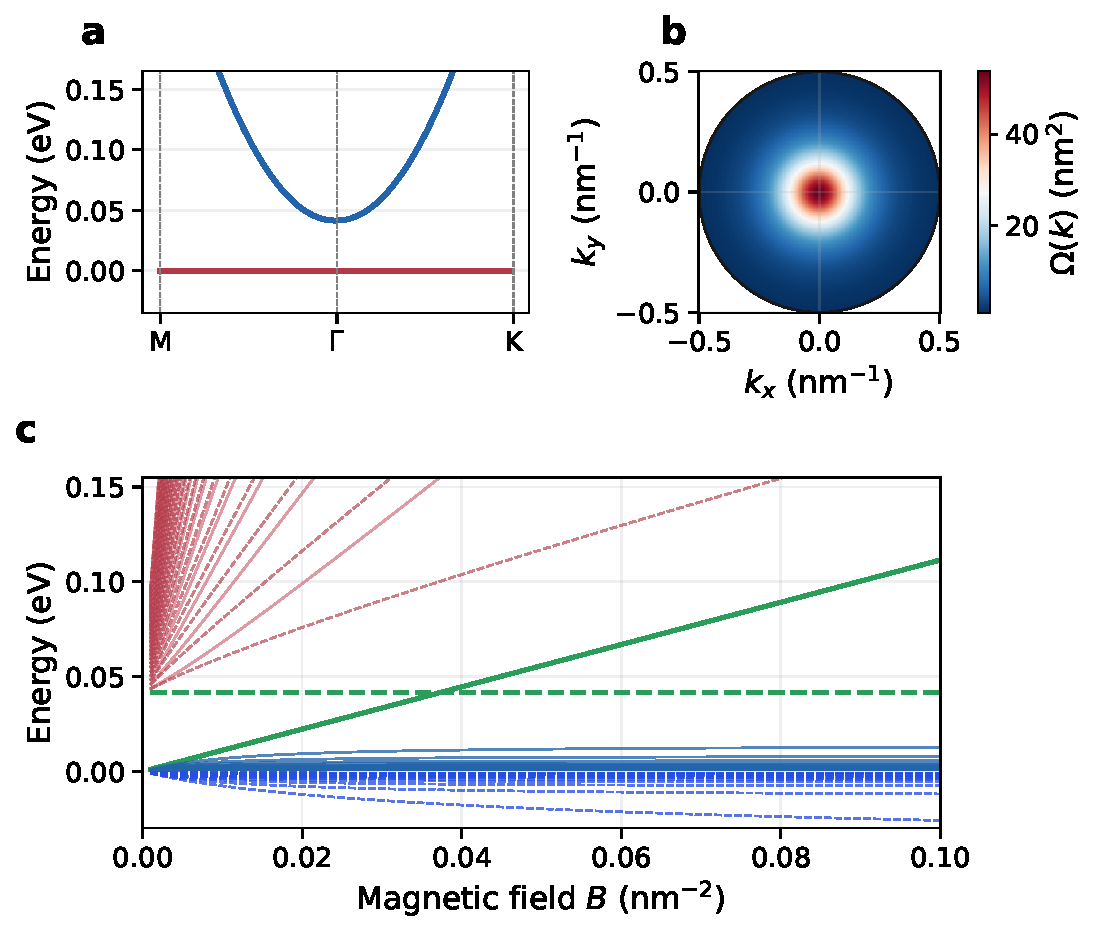
\includegraphics[width=\columnwidth]{../figures/manuscript figures/main_fig1_ideal_flatband_LL_spectrum.pdf}
	\caption{(a) Band dispersion at the ideal flat-band point along the $M$--$\Gamma$--$K$ path; the dispersive and flat bands are blue and red, respectively. (b) Berry-curvature distribution of the spin-up flat band. (c) Landau-level spectrum; normal, anomalous, and zeroth LLs are red, blue, and green, respectively, while solid and dashed curves distinguish the two spin sectors. Parameters: $a=1.115\,\mathrm{eV\cdot nm^2}$, $c=0.215\,\mathrm{eV\cdot nm}$, $E_0=0\,\mathrm{eV}$.}
	\label{fig:main1}
\end{figure}

%% ================================================================
%\section{LK Theory for Quantum Oscillations of Normal and Anomalous Landau Levels}
%\label{sec:lk-theory}
%% ================================================================
%
%\subsection{Local-spacing formulation of LK}

{\it Quantum oscillations of anomalous LLs - } We apply the standard LK
theory~\cite{lifshitz1956theory,shoenberg1984magnetic} to our model with both
normal and anomalous LLs (see SM Sec.~C) and derive the oscillatory part of the
grand potential as
\begin{equation}
\delta \Omega = \frac{D}{2\pi^{2}}\sum_{\alpha, \eta}\sum_{p=1}^{\infty}\frac{v_\mu^{\alpha,\eta}}{p^{2}} R_T \cos \bigl[2\pi p n^*_{\alpha,\eta}\bigr], \label{eq:omega-tilde}
\end{equation}
where $D = B/2\pi$ is the LL degeneracy, the LK thermal damping factor is given by
\begin{equation}
	R_T(p) = \frac{X_p}{\sinh X_p},\qquad
	X_p = \frac{2\pi^{2} p\, k_B T}{v_\mu^{\alpha,\eta}},
	\label{eq:Xp-manuscript}
\end{equation}
and the LL filling $n^*_{\alpha,\eta}$ is fixed by the chemical potential
$\mu$ through $E^\alpha_\eta(n^*_{\alpha,\eta},B) = \mu$.
Equations~(\ref{eq:omega-tilde}) and (\ref{eq:Xp-manuscript}) show that the
thermal damping is controlled by the local spacing $v_{\mu}^{\alpha,\eta}$ at
the chemical potential. In our numerical calculations, we fix the carrier
density $\rho$, which determines $\mu$ and $n^*_{\alpha,\eta}$ at each
magnetic field $B=e\mathcal{B}/\hbar$. The magnetization is evaluated as
$M=-(e/\hbar)\,\partial\Omega/\partial B$ at fixed $\rho$.

% Thus, the magnetization plotted below is reported in units of $\mathrm{eV}\,e/\hbar$, equivalently $\mathrm{eV\,nm^{-2}\,T^{-1}}$.

Figures~\ref{fig:main2}(a) and \ref{fig:main2}(b) show the magnetization
$M_{\mathcal{B}}$ as a function of $1/B$ for normal LLs in the electron-doped
regime, $\rho=+0.01\,\mathrm{nm}^{-2}$, and anomalous LLs in the hole-doped
regime, $\rho=-0.15\,\mathrm{nm}^{-2}$, respectively. Subtracting a smooth
background isolates the oscillatory magnetization in
Figs.~\ref{fig:main2}(c) and \ref{fig:main2}(d). The anomalous LLs retain
visible oscillations at high field, but their amplitude decays much more
rapidly than that of the normal LLs as $B$ decreases. The FFT peaks in
Figs.~\ref{fig:main2}(e) and \ref{fig:main2}(f) agree with the fundamental
counting frequency $F_{\rho}=2\pi|\rho_{\mathcal S}|$, where
$\rho_{\mathcal S}$ is the active-carrier density in the electron,
shallow-hole, or deep-hole sector (see SM Sec.~D). Although a Fermi-surface
area is not defined for the flat band, its oscillation frequency still follows
from LL counting: each filled LL accommodates $D=B/(2\pi)$ carriers per unit
area, so $n^*\simeq2\pi|\rho_{\mathcal S}|/B$. The agreement between the FFT
peaks and the dashed counting references therefore does not depend on a band
dispersion. Additional frequency diagnostics are presented in SM Sec.~D.


\begin{figure}[t]
	\centering
	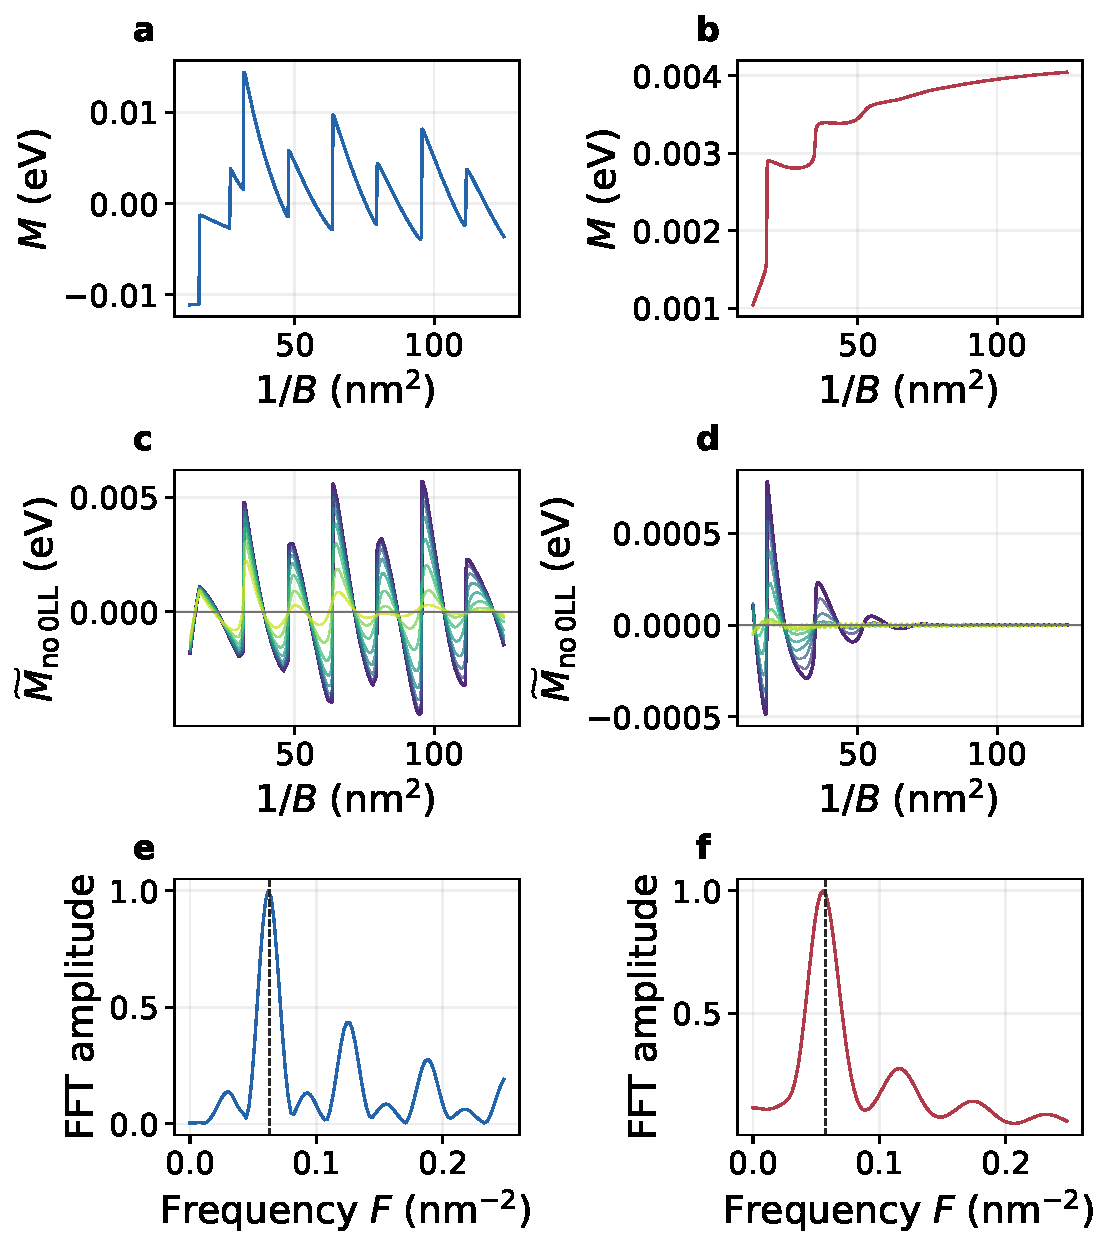
\includegraphics[width=\columnwidth]{../figures/manuscript figures/main_fig2_normal_anomalous_magnetization_oscillations.pdf}
	\caption{Fixed-density magnetization oscillations. (a) Full physical-field magnetization $M_{\mathcal{B}}$ in the normal regime, $\rho=+0.01\,\mathrm{nm}^{-2}$. (b) Full physical-field magnetization in the anomalous regime, $\rho=-0.15\,\mathrm{nm}^{-2}$. (c,d) Corresponding background-subtracted oscillatory magnetization at $k_B T=(2.00,\,3.07,\,4.71,\,7.22,\,11.1,\,17.0,\,26.1,\,40.0)\times10^{-4}\,\mathrm{eV}$, ordered from purple to yellow. (e,f) Corresponding normalized FFT spectra; dashed vertical lines mark the active-density counting frequency $F_{\rho}=2\pi|\rho_{\mathcal S}|$, measured in $\mathrm{nm}^{-2}$. Blue and red denote the normal and anomalous regimes, respectively.}
	\label{fig:main2}
\end{figure}

%
%
%% ================================================================
%\section{Thermal Damping of Quantum Oscillations for Normal and Anomalous Landau Levels}
%\label{sec:thermal-damping}
%% ================================================================

{\it Thermal damping and effective mass - } Finite temperature suppresses the
magnetization oscillations in Figs.~\ref{fig:main2}(c) and
\ref{fig:main2}(d). Because the signals are not perfectly sinusoidal, a global
Fourier transform does not cleanly isolate the thermal damping of individual
harmonics. We therefore use the short $1/B$ windows $W_0$, $W_1$, and $W_2$
marked in Figs.~\ref{fig:main3}(a) and \ref{fig:main3}(b), corresponding to
the first three complete high-field oscillation periods for the normal and
anomalous LLs. Within each window, we extract the amplitude $A_1$ of the
fundamental $p=1$ harmonic and plot $A_1(T)/A_1(T_{\min})$ in
Figs.~\ref{fig:main3}(c) and \ref{fig:main3}(d). The anomalous oscillations
show substantially stronger thermal damping. We fit this suppression with the
standard LK form using a single effective mass $\meff$:
\begin{equation}
	\frac{A_1(T)}{A_1(T_{\min})}
	= \frac{R_T(T,\meff,\bar{B}_w)}{R_T(T_{\min},\meff,\bar{B}_w)},\qquad
	X_1 = \frac{2\pi^{2} \kB T \meff}{\bar{B}_w},
	\label{eq:lk-fit}
\end{equation}
where $\bar{B}_w$ is the average magnetic field in the window. The dashed
curves in Figs.~\ref{fig:main3}(c) and \ref{fig:main3}(d) show that this
one-parameter form captures the qualitative damping trend in both regimes.
Comparing Eq.~(\ref{eq:lk-fit}) with Eq.~(\ref{eq:Xp-manuscript}) gives
\begin{equation}
	\meff(\bar{B}_w,\mu) = \frac{\bar{B}_w}{v_\mu^{\alpha,\eta}}, 
	\label{eq:meff-def}
\end{equation}
in units of $\mathrm{eV}^{-1}\mathrm{nm}^{-2}$. Figure~\ref{fig:main4}
summarizes the extracted masses. For the normal regime
($\rho=+0.01\,\mathrm{nm}^{-2}$), the fitted values are
$\meff\approx(0.626,\,0.788,\,0.958)\,\mathrm{eV}^{-1}\mathrm{nm}^{-2}$
across $W_0,W_1,W_2$ and remain comparatively small. In the anomalous regime
($\rho=-0.15\,\mathrm{nm}^{-2}$), they increase to
$\meff\approx(5.92,\,6.73,\,11.0)\,\mathrm{eV}^{-1}\mathrm{nm}^{-2}$ and
show a clear monotonic trend across the windows. The contrasting magnitude and
field dependence provide an experimental signature distinguishing anomalous
from normal LL oscillations.

The different trends can be understood from Fig.~\ref{fig:main1}(c). At large
$n^*$, the normal branches satisfy $(\mu-E_0)^2\gg c^2B$, whereas the
anomalous branches satisfy $(\mu-E_0)^2\ll c^2B$. The normal effective mass
then approaches the band-curvature value $\meff\approx1/(2a)$. For the
anomalous branches,
$\meff\approx c^2B/[2a(\mu-E_0)^2]$. At fixed carrier density, $n^*$ is
approximately fixed and $\mu-E_0\propto B$ in the anomalous regime, yielding
$\meff\sim1/B$. The dashed curves in Fig.~\ref{fig:main4} show these
analytical trends and agree qualitatively with the numerical results; the
derivation and additional tests are given in SM Secs.~C and D.

\begin{figure}[t]
	\centering
	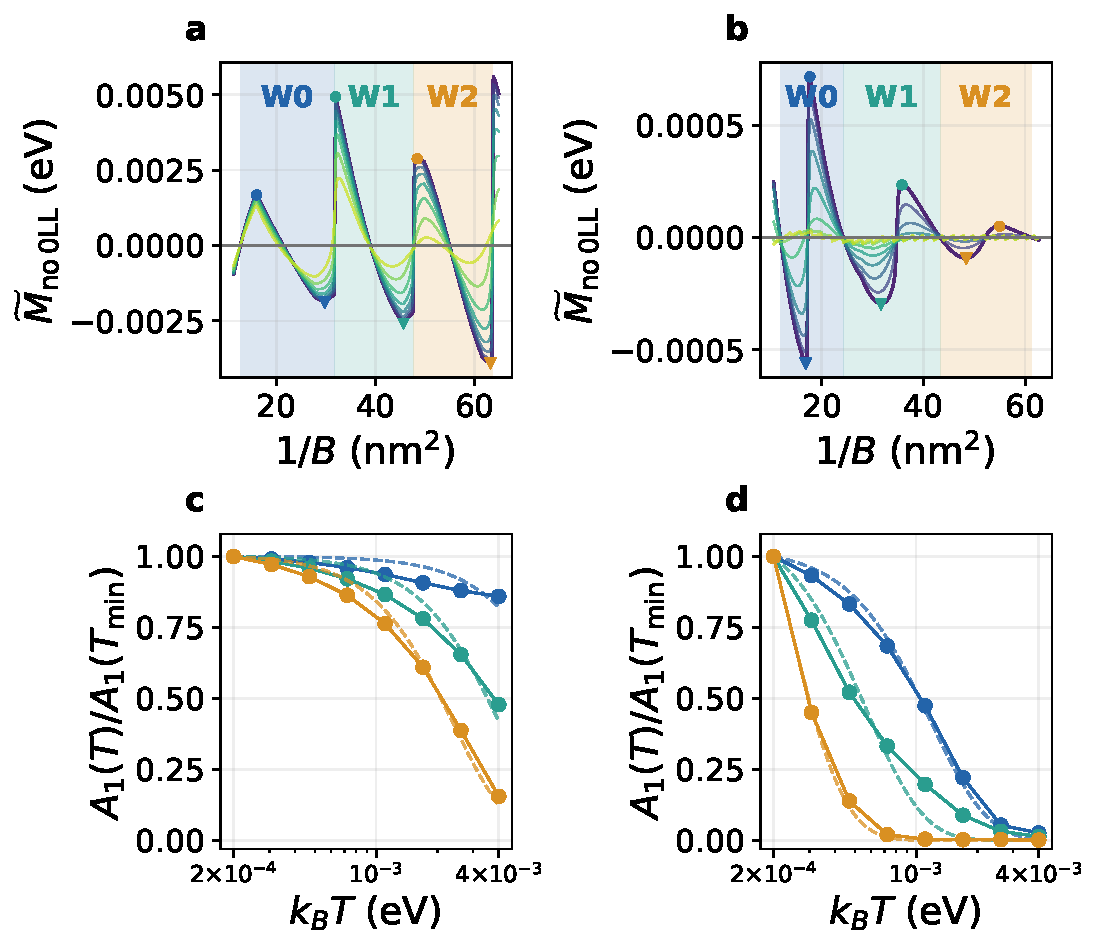
\includegraphics[width=\columnwidth]{../figures/manuscript figures/main_fig3_thermal_damping_local_windows.pdf}
	\caption{Thermal damping extracted from local oscillation windows. (a,b) Oscillatory magnetization in the normal regime, $\rho=+0.01\,\mathrm{nm}^{-2}$, and anomalous regime, $\rho=-0.15\,\mathrm{nm}^{-2}$, respectively, at $k_B T=(2.00,\,3.07,\,4.71,\,7.22,\,11.1,\,17.0,\,26.1,\,40.0)\times10^{-4}\,\mathrm{eV}$, ordered from purple to yellow. In (a,b), $W_0$, $W_1$, and $W_2$ are blue, teal, and orange, respectively. (c,d) Normalized $p=1$ harmonic amplitudes for the windows in (a,b), respectively; dashed curves are standard-LK fits.}
	\label{fig:main3}
\end{figure}


As the spreading of anomalous LLs is directly connected to quantum geometry of topological flat bands, we finally explore how to connect the effective mass $\meff$ to quantum geometric information. In the semi-classical limit with a large LL filling $n^*_{\alpha,-}\gg 1$, we find $U_{n^*} \approx V_{n^*} \approx a k_{n^*}^{2} + c^{2}/a$ with $k_{n^*}^{2} \approx 2n^*_{\alpha,-} B$. Consequently, we find the anomalous-branch local LL spacing $v_\mu^{\alpha,-} \approx \frac{2a c^{2} B^{2}}{(c^{2}/a + a k_{n^*}^{2})^{2}} = a B^{2} \tr\metric_\alpha(k_{n^*}) $ for both $\alpha = \uparrow, \downarrow$. This establishes the relationship between the effective cyclotron mass defined in Eq.(\ref{eq:meff-def}) and the quantum metric, 
\begin{equation}
	\meff \approx \frac{1}{a B\,\tr\metric_\alpha(k_{n^*})}. 
	\label{eq:meff-geometric}
\end{equation} 
Therefore, we demonstrate the magnetic field dependence of the effective mass for anomalous LLs is directly tied to the quantum metric of topological flat bands. 

\begin{figure}[t]
	\centering
	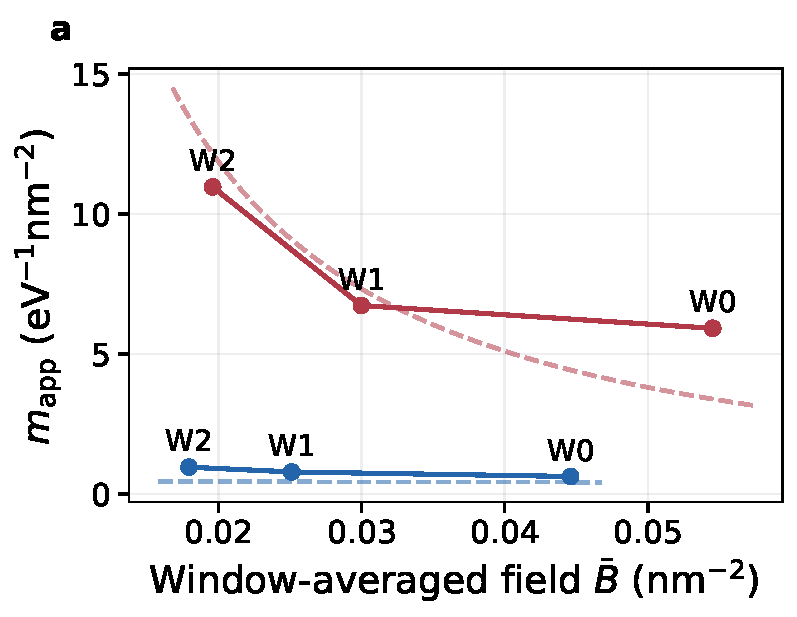
\includegraphics[width=\columnwidth]{../figures/manuscript figures/main_fig4_effective_mass_normal_anomalous.pdf}
	\caption{(a) Apparent effective mass, measured in $\mathrm{eV}^{-1}\mathrm{nm}^{-2}$, versus window-averaged magnetic field. Solid markers show masses extracted from the Fig.~\ref{fig:main3} damping fits for the normal regime, $\rho=+0.01\,\mathrm{nm}^{-2}$ (blue), and anomalous regime, $\rho=-0.15\,\mathrm{nm}^{-2}$ (red). Dashed curves show the corresponding analytical LK trends; labels identify the local windows.}
	\label{fig:main4}
\end{figure}



% % ================================================================
% \section{Conclusion}
% \label{sec:conclusion}
% % ================================================================

{\it Conclusion - } We have developed an LK description of quantum
oscillations from the anomalous Landau levels of ideal topological flat bands.
The oscillations remain finite because their thermal scale is set by the local
LL spacing rather than by a dispersion-derived cyclotron energy. In the
representative fixed-density comparison, the anomalous oscillations damp much
more rapidly than the normal oscillations and yield fitted effective masses
approximately an order of magnitude larger, with a pronounced field
dependence. In the semiclassical large-$n^*$ limit,
$\meff\sim1/[B\,\tr\metric]$, directly relating the damping scale to the
quantum metric. The frequency and the thermal scale thus play complementary
roles: LL counting fixes the oscillation period, while quantum geometry governs
the anomalous thermal damping. Given recent experimental progress in moir\'e
materials~\cite{cao2018unconventional,serlin2020intrinsic,cai2023signatures,zeng2023thermodynamic,xu2023observation,liu2022quantum},
temperature-dependent quantum-oscillation measurements offer a concrete route
to probing the quantum geometry of topological flat bands.

{\it Acknowledgments - }
We thank Zhen Bi and Jainendra Jain for helpful discussions. The author also acknowledges the use of Claude Code 2.1.200, OpenAI Codex CLI 0.140.0-alpha.2/GPT-5-based Codex, and TEXRA 0.39.2, directed through author-written prompts and author-provided manuscript/source files, for assistance with manuscript editing, code organization, numerical-code development, analytical derivation checks, reproducibility checks, and bibliography management; all AI-assisted code, calculations, derivations, references, scientific conclusions, and final manuscript content were independently checked by and remain the responsibility of the author. C.-X.L. acknowledges support from NSF grant DMR-2241327.

\bibliography{refs}

\end{document}
